% Chapter 1

\chapter{State of the Art}

\label{stateofart}

%----------------------------------------------------------------------------------------
\section{Music Genre Classification}

Music genre classification is a well-known objective and many different approaches exist to tackle it.
There have been numerous attempts at extracting genre information automatically from the audio signal, 
using signal processing techniques and machine learning schemes \cite{Aucouturier2003}.

Using this features different solutions have been proved to be efficient, 
including MLP or hierarchical classification in combination with a voting scheme \cite{Murauer2017}.

While these approaches work with low-level features and computations thereof, other solutions also take music theory into account.
Franklin \cite{Franklin2006} uses long short-term memory (LSTM) cells for extracting high-level features, which can subsequently be used for various
purposes. 

Li et al. \cite{Li2010} have shown that CNNs can be used for extracting features out of the raw audio data, which can then be used
for a variety of different tasks.
Other methods for genre prediction use spectrograms in combination with CNNs, transforming the task into an image classification
problem \cite{Gwardys2014}.

Finally, combinations of CNN and recurrent neural network
(RNN) models show improvements over the use of either solution
separately. 

Chen and Wang \cite{Chen2017} utilize three different CNNs for
different aspects of a spectrogram to calculate high-level descriptors,
which are subsequently fed into a LSTM-layer. 

Costa et al. \cite{Costa2017} use a CNN along with a SVM on hand-selected features from the
spectrogram image. They then combine these image predictions
with the outcome of a SVM trained on acoustical features by fusing
the results of both areas with different operations \cite{Murauer2018}.

Li et al. \cite{Li2003} propose a new method based on the Daubechies wavelet coefficients histograms
to improve the classification accuracy using Support Vector Machines and Linear Discrimination Analysis

%----------------------------------------------------------------------------------------

\section{MultiLabel Classification}

In multilabel classification, rather than multiclass classification, 
examples may belong to one or more set of classes. Regarding MLP there are several proposals.
Crammer and Singer \cite{Crammer2003} proposed Multi-label Multi-class Perceptron (MMP), a
family of on-line algorithms for ranking on text documents. 
One perceptron was used for each label but, unlike Bayesian Regression, the performance of the whole ensemble
was considered to update each perceptron. They showed that MMP outperformed
Bayesian Regression on text classification tasks.

The pairwise approach is often regarded as superior to Bayesain Regression because the former profits from simpler decision boundaries in the subproblems. 
Thus, while in MMP one perceptron was trained for each class, in \cite{Mencia2009}, multi-label pairwise perceptron (MLPP) was described with perceptrons as base classifiers. 
It was less efficient than MMP, but it resulted in a gain of accuracy.
In order to alleviate the complexity of this approach, quadratic with the number of labels, dual multi-label pairwise perceptrons algorithm (DMLPP) \cite{LozaMencia2008} formulated the perceptrons in dual form. 
Thus the prediction time depended linearly on the number of labels. 
Authors recommend this approach when the number of classes is high. 
Nevertheless, it is still less efficient than MMP and, as it keeps the whole training set in memory, it has problems to
handle training sets with many instances. 


On the contrary, MLPP is advisable if the number of classes is low and the number of examples high. 
Zhang and Zhou \cite{Zhang2006} developed Backpropagation for Multilabel Learning (BP-MLL), an adaptation of
the traditional multilayer feed-forward neural network. The key idea is the definition of an error function, closely related to the ranking loss.
The error function is minimised with gradient descent combined with the error
backpropagation.

The net has one input unit per input feature, one output unit
per label, and the hidden layer is fully connected with weights to the input and
output layers. Its computational complexity in the training phase is high, but the
time cost of predictions is quite trivial.


Multi Label Radial Basis Function (ML-RBF) \cite{Zhang2009} was inspired in the wellknown Radial Basis Function method. 
The first layer is obtained through k-means clustering on
instances of each possible class, the centre of each cluster being the prototype
vector of a basis function. Weights of the second layer were learnt by minimising
a sum-of-squares function \cite{Gibaja2014}.

%----------------------------------------------------------------------------------------

\section{Hierarchical Classification}

In hierarchical classification, examples are organised in a hierarchical
structure such as a tree or a directed acyclic graph (DAG), which allows a child
category to have more than one parent category. 

This entails several challenges.
First, classes in the bottom of the hierarchy tend to be more difficult to identify
because the number of samples is usually less than in upper classes. 
Secondly, the closer a category is to the root, the more a wrong decision affects lower levels. And
finally, predictions must respect the class hierarchy. 

\begin{figure}[th]
    \centering
    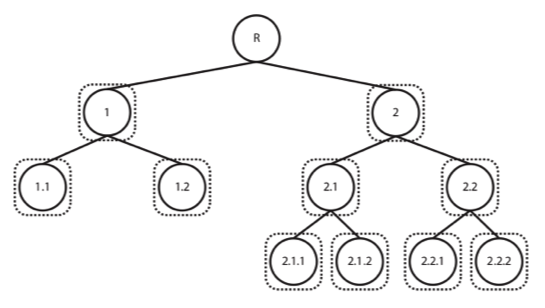
\includegraphics[width=1.0\textwidth]{Figures/hierachical.png}
    \decoRule
    \caption[Hierarchical Classification example]{Hierarchical Classification example (Image credit \cite{Silla2011})}
    \label{fig:hierachical}
\end{figure}

Thus, according to the true path rule, an example that belongs to some class automatically belongs to all its ancestors,
and negative predictions for a given node are propagated to the descendants to
preserve the consistency of the hierarchy. 

Typical examples of hierarchical domains
are protein function prediction and text categorization.
In \cite{Cerri2012} and \cite{Silla2011} two approaches for hierarchical multi-label classification are
described: the local one (top-down) consists of training a hierarchy of classifiers, which are used in a top-down fashion for the classification of new examples; and the global one (one-shot, big-bang), that induces
a unique classifier using all classes of the hierarchy at once and is able to predict just in one step. 

On the other hand, three baseline approaches were identified in \cite{Vens2008}, the two first corresponded to local methods and the last one corresponded
to global methods: Single-label Classification approach (SC), Hierarchical Singlelabel Classification (HSC) and Hierarchical Multi-label Classification (HMC).
SC trains a binary classifier for each label in the hierarchy considering as
positive examples those labelled with such class and the rest are considered to be
negative. This approach has several drawbacks. 

First, it needs to train one classifier per class (which can be hundreds or thousands). 
Besides, as the hierarchy is not taken into account, it is also possible having inconsistencies. 
Finally, it is very likely having a problem of imbalanced data at lower levels of the hierarchy with only a few positive patterns and too many negative ones \cite{Gibaja2014}.


%----------------------------------------------------------------------------------------

\section{Related Work}

Since the problem faced in this paper is a yearly contest held by the AcousticBrainz project \cite{genretask} 
some several contestants and applications submit their solutions with different approaches and algorithms to tackle this problem.

Koutini et al. \cite{koutinimediaeval} used a simple MLP to recognize the genres.

Schreiber, H \cite{schreiber2018mediaeval} used a CNN network alongside the provided Mel features.

Oramas et al. in \cite{oramas2018mediaeval} propose two different approaches using all the available low level features.

%----------------------------------------------------------------------------------------
